\documentclass[tikz,border=8pt]{standalone}
% Shared preamble of the task figures of Lecture 8. The colours are the slide colour roles of Lectures 6 to 8
% (and of the signatures simulator):
%   Alice and her keys and signature: indigo (private key and signature full, public key light),
%   Eve and Mallory: pink, the message: violet, the shared MAC key: amber, Bob and the verifier: teal,
%   the digest and the MAC tag: brown, mechanisms: dark neutral, an unknown result: orange "?".
\usepackage{lmodern}
\usepackage[T1]{fontenc}
\renewcommand{\familydefault}{\sfdefault}
\usepackage{amsmath,amssymb}
\usepackage{xcolor}
\usepackage{fontawesome5}
\usetikzlibrary{arrows.meta, calc, positioning, fit, decorations.pathmorphing}

\definecolor{DeepBlue}{HTML}{283593}
\definecolor{AccentOrange}{HTML}{EB5A14}
\definecolor{nInk}{HTML}{37474F}
\definecolor{nLine}{HTML}{90A4AE}
\definecolor{nLight}{HTML}{CFD8DC}
\definecolor{nFill}{HTML}{ECEFF1}
\definecolor{aExec}{HTML}{43A047}
\definecolor{aWrite}{HTML}{E53935}
\definecolor{sIndigo}{HTML}{5C6BC0}
\definecolor{sPink}{HTML}{EC407A}
\definecolor{sViolet}{HTML}{7E57C2}
\definecolor{sAmber}{HTML}{FFB300}
\definecolor{sTeal}{HTML}{26A69A}
\definecolor{sBrown}{HTML}{8D6E63}
\definecolor{sPinkText}{HTML}{C2185B}

\tikzset{
  hw/.style={draw=nLine, thick, fill=nFill, text=nInk, rounded corners=3pt, align=center, inner sep=4pt},
  hwmain/.style={draw=nInk, thick, fill=nInk, text=white, rounded corners=3pt, align=center, inner sep=5pt, font=\small\bfseries},
  msg/.style={draw=sViolet, thick, fill=sViolet!15, text=nInk, rounded corners=3pt, align=center, inner sep=4pt},
  digest/.style={draw=sBrown, thick, fill=sBrown!15, text=nInk, rounded corners=3pt, align=center, inner sep=4pt},
  mackey/.style={draw=sAmber, thick, fill=sAmber!30, text=nInk, rounded corners=3pt, align=center, inner sep=4pt},
  apriv/.style={draw=sIndigo, thick, fill=sIndigo, text=white, rounded corners=3pt, align=center, inner sep=4pt},
  apub/.style={draw=sIndigo, thick, fill=sIndigo!15, text=nInk, rounded corners=3pt, align=center, inner sep=4pt},
  asig/.style={draw=sIndigo, thick, fill=sIndigo, text=white, rounded corners=3pt, align=center, inner sep=4pt},
  mpriv/.style={draw=sPink, thick, fill=sPink, text=white, rounded corners=3pt, align=center, inner sep=4pt},
  mpub/.style={draw=sPink, thick, fill=sPink!15, text=nInk, rounded corners=3pt, align=center, inner sep=4pt},
  unk/.style={draw=AccentOrange, thick, dashed, fill=white, text=AccentOrange, rounded corners=3pt, align=center, inner sep=4pt, font=\bfseries},
  data/.style={-{Stealth}, very thick, nInk},
  person/.style={circle, fill=#1, draw=#1, text=white, minimum size=1.0cm, font=\large, inner sep=0pt},
  pname/.style={font=\small\bfseries, text=nInk},
  net/.style={-{Stealth}, very thick, nInk, decorate, decoration={snake, amplitude=1.4pt, segment length=8pt, post length=4pt}},
}
% \who{node}{pos}{colour}{icon}{name}
\newcommand{\who}[5]{\node[person=#3] (#1) at (#2) {#4}; \node[pname, below=1pt of #1] {#5};}

\begin{document}
\begin{tikzpicture}[>=Stealth]
\who{A}{0,0}{sIndigo}{\faUser}{Alice}
\node[msg, font=\small] (o1) at (3.0,0.6) {20 pounds};
\node[asig, font=\scriptsize\ttfamily] (s1) at (6.4,0.6) {80a9b014e367\ldots 069ba6863a16};
\node[msg, font=\small] (o2) at (3.0,-0.6) {50 pounds};
\node[asig, font=\scriptsize\ttfamily] (s2) at (6.4,-0.6) {c95f1a1e8b14\ldots 5617ecb95454};
\draw[data] (A) -- (o1.west); \draw[data] (A) -- (o2.west);
\draw[data] (o1) -- (s1); \draw[data] (o2) -- (s2);
\who{M}{0,-2.8}{sPink}{\faUserSecret}{Mallory}
\node[mpriv, font=\small] (f) at (3.6,-2.6) {sig\_1 $\times$ sig\_2 mod n};
\node[msg, font=\small] (o3) at (7.2,-2.6) {1000 pounds};
\node[unk] at (9.4,-2.6) {bank: ?};
\node[mpriv, font=\small] (r) at (3.6,-3.6) {any number: 123\,456\,789};
\node[unk] (ra) at (7.2,-3.6) {amount = ?};
\node[unk] at (9.4,-3.6) {bank: ?};
\draw[data] (M) -- (f.west); \draw[data] (M) -- (r.west); \draw[data] (f) -- (o3); \draw[data] (r) -- (ra);
\node[hw, font=\scriptsize] at (11.6,-0.9) {\faUniversity\ Alice's bank\\ accepts s if\\ s\textsuperscript{e} mod n = amount};
\end{tikzpicture}
\end{document}
